%%%%%%%%%%%%%%%%%%%%%%%%%%%%%%%%%%%%%%%%%%%%%%%%%%%%%%%%%%%%%%%%%
%  _____       ______   ____									%
% |_   _|     |  ____|/ ____|  Institute of Embedded Systems	%
%   | |  _ __ | |__  | (___    Wireless Group					%
%   | | | '_ \|  __|  \___ \   Zuercher Hochschule Winterthur	%
%  _| |_| | | | |____ ____) |  (University of Applied Sciences)	%
% |_____|_| |_|______|_____/   8401 Winterthur, Switzerland		%
%																%
%%%%%%%%%%%%%%%%%%%%%%%%%%%%%%%%%%%%%%%%%%%%%%%%%%%%%%%%%%%%%%%%%

\chapter{\textit{glitches}}\label{chap.glitch}

\section{Definition Glitches}\label{sect.glitch_def}

Im technischem Bereich bedeutet gemäss Cambridge Dictionaire ein \textit{glitch}, eine ungewollte, flüchtige Signalspitze, die ein Fehlverhalten im System verursacht. Im Anhang  befindet sich der Originaltext wie auch noch eine weitere Defintion aus dem englischen Sprachraum.

In der digitalen Signalverarbeitung ist das Glitch ein bekannter Begriff und wird dort unter anderem leicht sarkastisch beschrieben:

\textit{''Als ''Glitch''  wird eine ungewollte, flüchtige ''Signalspitze'' bezeichnet, die Zähler aufwärts zählt, Register löscht oder einen ungewollten Prozess startet.}'' 
\cite{F_glitches}


Am intuitivsten ist die bildliche Darstellung des soeben beschriebenen Fehlverhaltens (Abbildung \ref{fig.glitch.def}). In dieser Signalabfolge treten zwei mal Glitches auf, die eigentlich nicht dort hingehören.\\
\todo{besseres Bild def Glitch}
\begin{figure}[H]
	\centering
	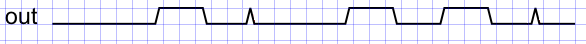
\includegraphics[width=\textwidth]{images/glitch/def_glitch_1.png}
	\caption{Glitch-Signalspitzen}
	\label{fig.glitch.def}
\end{figure}

Auf den ersten Blick scheinen solch temporäre Spannungsspitzen nicht zu stören. Doch wenn man Pech hat, sind Glitches der Auslöser für Abstürze oder zumindest für ein Fehlverhalten eines Gerätes. Aus diesem Grund, wird nun der Ursache dieser Spitzen nachgegangen.\\ 



\section{Ursache für Glitches}\label{sect.glitch_ursache}
Der Auslöser der flüchtigen Spannungsspitzen sind asynchrone Inputs vor einem asynchronen Bauteil oder verzögerte Signale. Trifft z. B. vor einem Dekoder von vier Leitungen, das Signal einer Leitung zu spät an, entschlüsselt der Dekoder kurzfristig einen falschen Wert. Obwohl die Störung nur kurz ist, übermittelt ein asynchroner den falschen Wert direkt an seinen Ausgang. \\

\subsection{Asynchroner Input}
Das ungleichzeitige Eintreffen von Signalen kann z.B. durch lange Signalpfade (Leitungen), unterschiedliche Durchlaufverzögerungen der vorangehenden Flip-Flops oder unterschiedliche Logik-Zeiten entstehen. Grundsätzlich gelten alle nicht-getakteten Prozesse als potenzielles Risiko für Glitches, da man bei ungetakteten Prozessen nicht weiss, wie lange sie dauern.\\

\subsection{Nachteil getakteter Prozesse}
Jeder getaktete Prozess verzögert die Verarbeitung. Aus diesem Grund wird abgewogen, wo Prozesse getaktet und wo sie asynchron getätig werden. In VHDL gibt es viele asynchrone Vorgänge (wie ungetaktete Prozesse oder Singalzuweisungen), deshalb ist es vorteilhaft, wenn das Risiko asynchroner Prozesse bekannt ist.\\


Abbilung \ref{fig.glitch.bild1} zeigt ein leicht verzögertes (getaktetes) enable-Signal zu einem anders verzögerten (getakteten) Flip-Flop-Eingangssignal Q. Der Ausgang des Flip-Flops weist kurzzeitig Glitches auf. \\
\begin{figure}[H]
	\centering
	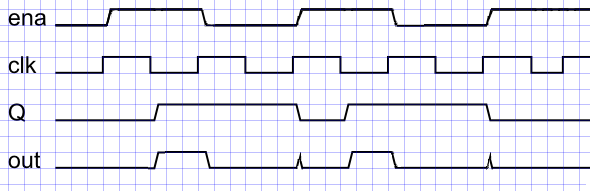
\includegraphics[width=0.8\textwidth]{images/glitch/def_glitch_3.png}
	\caption{Mögliches Bsp. für Glitches}
	\label{fig.glitch.bild1}
\end{figure}



\section{Glitches erzeugen}\label{sect.glitch_detect}
Was in Glitch ist, ist relativ einfach zu beschreiben. Ein Glitch jedoch mit moderner Digitaltechnik  zu erzeugen, erweist sich als etwas schwerer. Hier zwei Ansätze, die getestet werden. \\

\subsection{Glitches Aufgrund von Bauteiltoleranzen}\label{sect.glitch_toleranzen}

Der erste Ansatz ist, ein Zähler aus vier Flipflops mit asynchronem Dekoder zu implementieren. 

\subsubsection{Konzept}
Die Erwartung ist, dass aufgrund der \textit{Bauteiltoleranzen} der Flip-Flops die vier Ausgänge an den Flip-Flops nicht gleichzeitg ihren Wert übermitteln. Die einen sind leicht schneller, die anderen leicht verzögert. Dadurch ergibt sich kurzzeitig am asynchronen Dekoder einen falschen Wert.\\
Damit ein abnormaler Wert in einem Zähler erkannt wird, sendet der Dekoder bei der Zahl 7 einen Peak. Ohne Glitch entschlüsselt der Dekoder in regelmässigen Abständen von 160 ns diese Zahl. Aufgrund der Flip-Flop-Bauteiltolereanzen ist ein kurzzeitiges Dekodieren einer 7 \textit{ausserhalb der Periode T} zu erwarten. 
\begin{figure}[H]
	\centering
	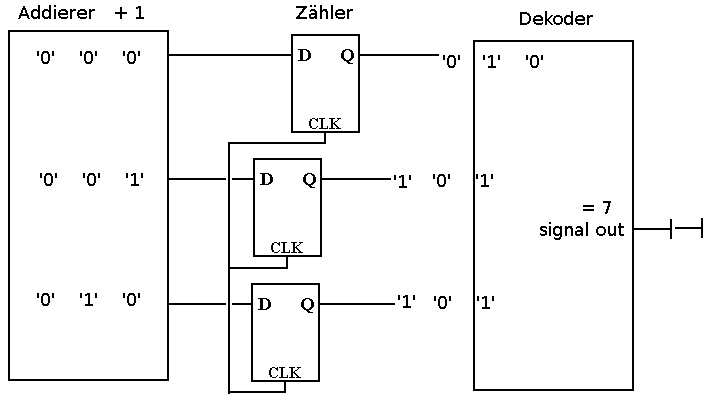
\includegraphics[width=0.6\textwidth]{images/glitch/Ansatz_1.png}
	\caption{Ausnutzen der Bauteilverzögerung}
	\label{fig.glitch.counter3}
\end{figure}


\subsubsection{Implementation}
\todo{Bild anpassen}
\begin{figure}[H]
	\centering
	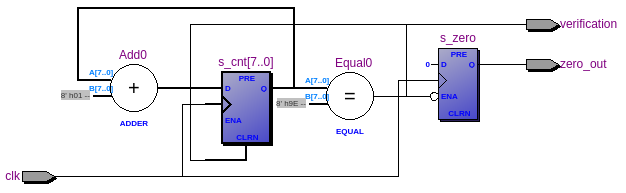
\includegraphics[width=\textwidth]{images/glitch/RTL_counter_2.png}
	\caption{RTL Zahler mit asynchronem Dekoder}
	\label{fig.glitch.counter2}
\end{figure}
\todo {Bild Asynchronem Zähler besser beschreiben}

Um die gewollten Zahlenwerte von den Glitches zu unterschieden, wird das asynchrone Singnal getaktet. Dadurch erscheint der korrekte Zählwert mit einem Takt Verzögerung. Die Periode ist 20 ns (CLK = 50 MHz).\\





\subsection{Glitches Aufgrund von Pfadverzögerung}\label{sect.glitch_toleranz}
Der zweite Ansatz ist die gesuchte Bauteilverzögerungen über längere Signalpfade zu simulieren.Der Dekoder des Zählers bleibt asynchron. 

\subsubsection{Konzept}
Dekodiert wird die Zahl 15. Durch intelligentes Routing (FF 1 wird verzögert, FF 2 wird beschleunigt) wird der Zustand der Zahl 11 forcier \todo {Bild FF1 verzögert, FF2 schneller}

\subsubsection{Implementation} 
Cyclone II, Board De2. Quartus 13.0sp.

Die Pfad\textit{verlängerung} wird über das Routing über die GPIO-Pins des Headers 1 gemacht (siehe Abbildung \ref{fig.glitch.routing}. Die obersten vier Doppel-Pins erhalten eine "Brücke", sodass das Signal links ausgegeben und rechts wieder eingespiesen wird.\\
Signal\textit{verkürzung} ist eine direkte Signalzuweisung \todo {korrektes Wort ?(Concourent Assignment)} .\\
\begin{figure}[H]
	\centering
	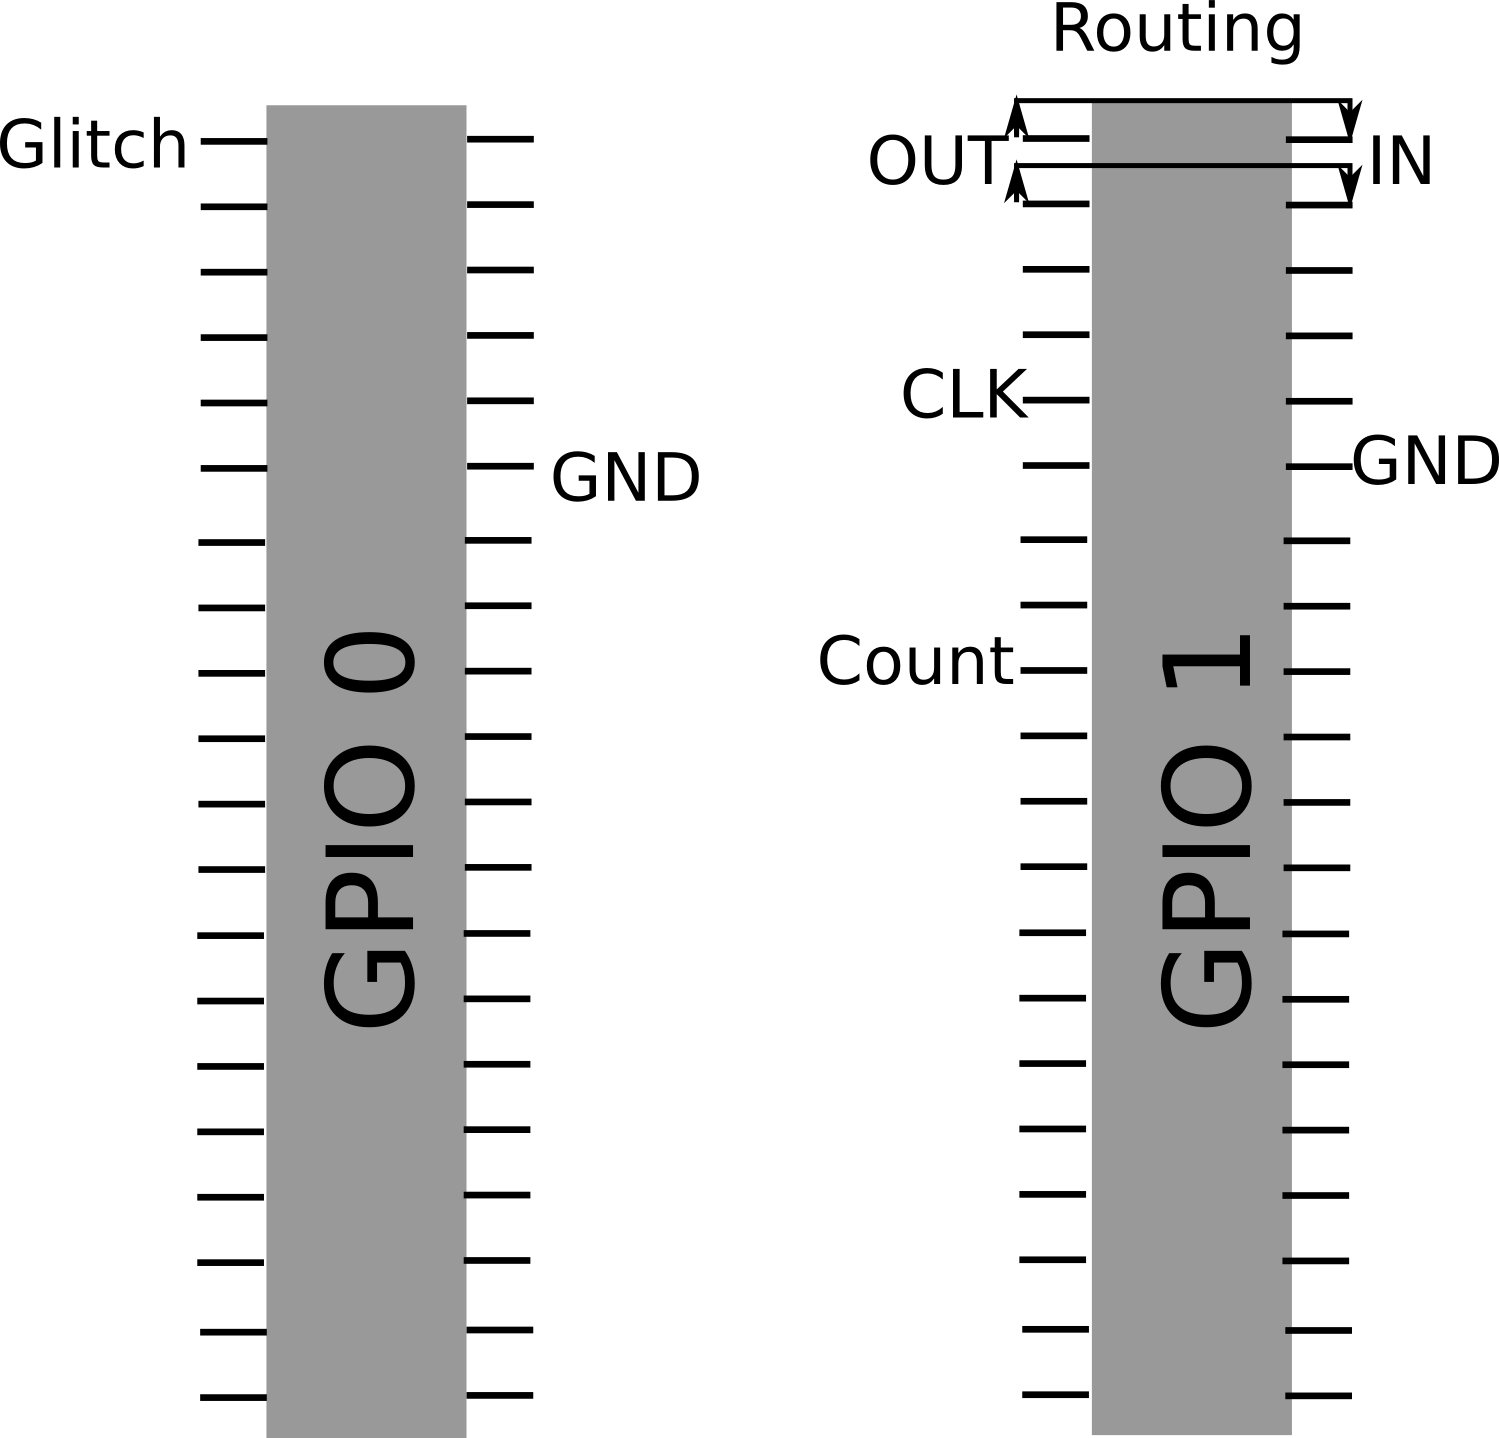
\includegraphics[width=0.3\textwidth]{images/glitch/GPIO_Belegung.png}
	\caption{GPIO Anschlüsse}
	\label{fig.glitch.GPIO}
\end{figure}

Auf dem KO wird das asynchrone Glitch-Signal und das synchrone Zählersignal neben dem Takt ausgegeben. Weil der Zähler synchronisiert wurde, ist der Wert 1 Periode (= 20 ns) später als der Glitch.\\

\begin{figure}[H]
	\centering
	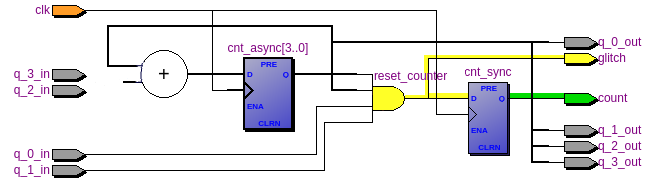
\includegraphics[width=\textwidth]{images/glitch/RTL_glitch_detection_bemalt.png}
	\caption{Zähler mit Signal-Routing über GPIO}
	\label{fig.glitch.routing}
\end{figure}
Im RTL-Diagramm sieht man deutlich den Unterschied zwischen dem asynchronen Zähler, der über das Gate \textit{reset\_{counter}} beim Wert 15 einen Impuls an den Ausgang glitch gibt und dem synchronisierten Zähler \textit{cnt\_{sync}} der dem asynchronen Ausgang nachgeschaltet ist und dieses Signal taktet. Das getaktete Zähl-Signal geht an den Ausgang \textit{count}.


	
\section{Resultat Glitches provozieren}\label{sect.glitch_resultat}

\subsection{Erzeugen über Bauteiltoleranzen}
Der Ansatz, dass die Bauteiltoleranzen der Flip-flops eine Ursache für asynchrone Inputs in den Dekoder sind ist korrekt. Die Umsetzung zeigte sich jedoch als schwierig, da die heutigen Flip-Flops zu schnell sind bzw. ihre Toleranzen zu klein um sichtbar zu werden. \todo {Timeanalyse für FF} Aus diesem Grund entschlüsselte der asynchrone Dekoder trotz kleinen Verzögerungen die Werte stets korrekt.\\



\subsection{Erzeugen über Routing} 
\begin{figure}[H]
	\centering
	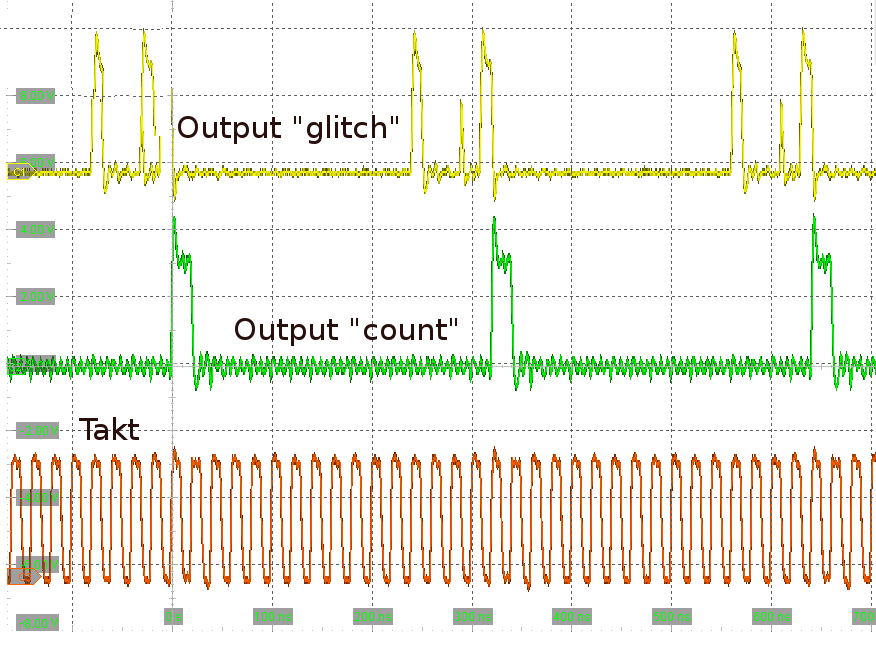
\includegraphics[width=0.8\textwidth]{images/glitch/Glitch_2_good_kommentar.png}
	\caption{Glitch (gelb), Zähler (grün) und Takt (orange)}
	\label{fig.glitch.result_1}
\end{figure}

Typisch ist, dass der synchrone Zähler eine Signalbreite von genau einer Periode hat, da dieses Signal getaktet ist. Dagegen hat der asynchrone Glitch keine konstante Breite.
\begin{enumerate}
	\item{Bei welchen Zählständen treten Glitches auf?}

	\item{Wie hängen die Zählständen mit dem gewählten Routing zusammen?}

\end{enumerate}
